\documentclass[a4paper]{article}

\setlength{\voffset}{-15mm}
\setlength{\textheight}{230mm}
\setlength{\hoffset}{-10mm}
\setlength{\textwidth}{157mm}

\usepackage{CJK}
\usepackage{graphicx}

\begin{document}
    \begin{center}
        \textsf{\LARGE{Quantum Mechanics (A) - Assignment 5}}\\[20pt]
    \end{center}
    
    \noindent\Large{\emph{October 9 , 2014}}\\[15pt]
    \begin{CJK*}{UTF8}{song}
    2.2 \textbf{证明:}\\[12pt]
    {
     根据《量子力学教程》[2nd,曾谨言]-2.2.1 p31-32
    \[\psi_{n}(x) =\left\{
    \begin{array}{ll}
        \displaystyle\sqrt{\frac{2}{a}} \sin(\frac{n \pi x}{a}) \quad  ,  \quad 0 < x < a\\[12pt]
        \quad 0 \quad  ,  \quad x<0,x>a
    \end{array}
    \right.
    \]
    则由期望值公式可得
    \begin{eqnarray}
        \overline{x_{n}} & = & \int_{-\infty}^{\infty}x |\psi (x)|^{2} \mathrm{d x}\nonumber\\[5pt]
                     & = & \int_{0}^{a}x ( \frac{2}{a} sin^{2} (\frac{n \pi x}{a}) ) \mathrm{d x} \nonumber\\[5pt]
                     & = & \frac{a}{2} \nonumber
    \end{eqnarray}
    \begin{eqnarray}
        \overline{x^{2}_{n}} & = & \int_{-\infty}^{\infty}x^{2} |\psi_{n} (x)|^{2} \mathrm{d x}\nonumber\\[5pt]
            & = & \int_{0}^{a}x^{2} ( \frac{2}{a} sin^{2} (\frac{n \pi x}{a}) ) \mathrm{d x} \nonumber\\[5pt]
            & = & \frac{a^{2}}{3} (1 - \frac{3}{2 n^{2} {\pi}^{2}}) \nonumber
    \end{eqnarray}
    由方差公式
    \setcounter{equation}{1}
    $$\overline{( x - \overline{x})^{2}} = \overline{x^{2}} - \overline{x}^{2}
        = \frac{a^{2}}{12} ( 1 - \frac{6}{n^{2} {\pi}^{2}})$$ \\[8pt]
    \begin{CJK*}{UTF8}{kai}
    \noindent \textbf{*讨论$n\rightarrow\infty$的情况,并与经典力学计算结果比较.}\\[15pt]
    \end{CJK*}
    经典力学中,粒子在允许区内随机均匀分布,即 $\displaystyle P(x)=\frac{1}{a}$
    $$
        \overline{x}  =  \int_{-\infty}^{\infty}x P(x) \mathrm{d x}
                      =  \int_{0}^{a}x \frac{\mathrm{d x}}{a}
                      =  \frac{a}{2} \nonumber
    $$
    \begin{eqnarray}
        \overline{x^{2}}  =  \int_{-\infty}^{\infty}x^{2} P(x) \mathrm{d x}
             =  \int_{0}^{a}x^{2} \frac{\mathrm{d x}}{a}
             =  \frac{a^{2}}{3} \nonumber
    \end{eqnarray}
    $$ \overline{( x - \overline{x})^{2}} = \overline{x^{2}} - \overline{x}^{2}
        = \frac{a^{2}}{12}$$ \\[8pt]
    当$n\rightarrow\infty$时,由式(1)得
    $$\lim_{n\rightarrow\infty} \overline{( x - \overline{x})^{2}} 
        = \lim_{n\rightarrow\infty} \frac{a^{2}}{12} ( 1 - \frac{6}{n^{2} {\pi}^{2}}) = \frac{a^{2}}{12}
        $$
    与经典力学计算结果一致\\[15pt]      
    \begin{CJK*}{UTF8}{kai}
    \noindent\textbf{*计算$\Delta p$和$\Delta x\cdot\Delta p.$}
    \end{CJK*}
    \\[15pt] 根据变换公式可得
    \begin{eqnarray}
        \varphi_{n}(p) & = & \frac{1}{\sqrt{2\pi\hbar}} \int_{-\infty}^{\infty}\psi_{n}(x) e ^{ - i p x / \hbar}\mathrm{d x}\nonumber \\[7pt]
            & = & \frac{1}{\sqrt{2\pi\hbar}} \int_{0}^{a} \sqrt{\frac{2}{a}} \sin (\frac{n \pi x}{a})\cos (\frac{p}{\hbar} x) \mathrm{d x}\nonumber\\[7pt]
                & = & n \sqrt{\pi a \hbar^{3}}
                \frac{1 - (-1)^{n} \cos (\frac{a p}{\hbar}) }{n^{2} {\pi}^{2} {\hbar}^{2} - a^{2} p^{2}} \nonumber
    \end{eqnarray}
    代入公式计算期望值
    $$\overline{p_{n}} = \int_{-\infty}^{\infty} p |\varphi_{n}(p)|^{2} \mathrm{d p} = 0 $$
    $$\overline{p_{n}^{2}} = \int_{-\infty}^{\infty} p^{2}\cdot |\varphi_{p}|^{2} \mathrm{d p}
        = \frac{3 n^{2} {\pi}^{2} {\hbar}^{2}}{a^{2} ( 1 - 6/n^{2}{\pi}^{2})}
        $$
    $$\Delta p = \sqrt{\overline{x-\overline{x}}^{2}} = \sqrt{\overline{x^{2}}-\overline{x}^{x}}
        = \frac{n \pi \hbar}{a}\sqrt{\frac{3}{n^{2} {\pi}^{2} - 6}}
        $$
    $$\Delta x \cdot \Delta p =
        \sqrt{\frac{a^{2}}{12}(1-\frac{6}{n^{2}{\pi}^{2}})}
        \cdot
        \frac{n \pi \hbar}{a}\sqrt{\frac{3}{n^{2} {\pi}^{2} - 6}}
        = \frac{\hbar}{2}
        $$
    }\\[20pt]
    \noindent 2.3 \textbf{解:}\\[12pt]
    {
    根据《量子力学教程》[2nd,曾谨言]-2.2.1 p32-33
     $$\mbox{基态} \quad \psi_{1}(x) = \sqrt{\frac{2}{a}}\cos(\frac{\pi x}{a})$$
    概率密度分布函数
    \begin{eqnarray}
        \varphi_{1}(p) & = & \frac{1}{\sqrt{2\pi\hbar}} \int_{-\infty}^{\infty}
        \psi_{n}(x) e ^{ - i p x / \hbar}\mathrm{d x}\nonumber \\[7pt]
            & = & \frac{1}{\sqrt{2\pi\hbar}} \int^{a/2}_{-a/2}
            \sqrt{\frac{2}{a}}\cos (\frac{\pi x}{a})\cos (\frac{p x }{\hbar})\mathrm{d p}\nonumber\\[7pt]
                & = &  2\sqrt{\pi a \hbar^{3}} \cdot \frac{\cos (p a /2\hbar)}{\pi^{2}\hbar^{2} - p^{2}a^{2}}\nonumber
    \end{eqnarray}
    概率分布函数
    $$|\varphi_{1}(p)|^{2} =
        2\pi a \hbar^{3} \cdot \frac{\cos^{2}(p a /2\hbar)}{(\pi^{2}\hbar^{2} - p^{2}a^{2})^{2}}
        $$
    }\\[20pt]
    \noindent 2.4 \textbf{解:}\\[12pt]
    {
    \noindent (a) \quad 根据归一化条件
    $$\int_{-\infty}^{\infty} |\psi (x)|^{2} \mathrm{d x}
        = \int_{0}^{a} [A x ( a - x)]^{2} \mathrm{d x}
        = 1 \quad \mbox{即} \quad A = \sqrt{\frac{30}{a^5}}
        $$
    \noindent (b)\quad$\psi (x)$用$\psi_{n}(x)$展开
    $$\psi (x) = \sum C_{n} \psi_{n}(x)$$
    \begin{eqnarray}
        C_{n} & = & \int \psi_{n}^{*} (x) \psi (x) \mathrm{d x}
        =  \int_{0}^{a} \sin (\frac{n \pi x}{a}) \sqrt{\frac{30}{a^{5}}} x (a - x) \mathrm{d x}\nonumber\\
            & = & \frac{4\sqrt{15}}{n^{2} \pi^{3}}[1 - (-1)^{n}]\nonumber\\
        P_{n} & = & |C_{n}|^{2} = \frac{240}{n^{6} \pi^{6}}[1 - (-1)^{n}]^{2}\nonumber
    \end{eqnarray}
    特别的,基态$\displaystyle P_{1}=\frac{960}{\pi^{6}} \approx 0.99855.$\\[8pt]
    \noindent (c)\quad 作图比较$\psi_{1}(x)$和$\psi (x)$\\[8pt]
    \begin{figure}[ht]
      \centering
      % Requires \usepackage{graphicx}
      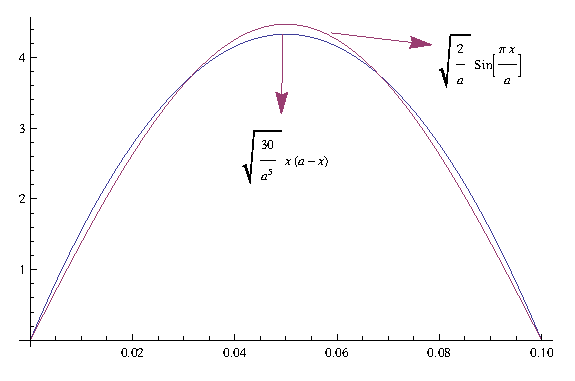
\includegraphics[width=300pt,height=200pt]{figure2.eps}\\
      \caption{$\psi(x,0) vs \psi_{1}(x)$}
    \end{figure}
    由图可见,$\psi_{1}(x)$和$\psi (x)$曲线基本重合,\\
    又简单计算比较有: 
    $$\displaystyle \frac{P_{n}}{P_{1}}(n \neq 1)<\frac{1- P_{1}}{P_{1}} = \frac{1 - 0.99855}{0.99855} \approx 1.4 \times 10^{-3} \ll 1
        \mbox{即}
        \displaystyle P_{n}|_{n\neq 1}\ll P_{1}
        $$
    由此可知$\psi_{1}(x)$和$\psi (x)$几乎一致。
    }\\[40pt]  
    \Large{\emph{October 13 , 2014}}\\[15pt]
    \begin{CJK*}{UTF8}{kai}
    \noindent \textbf{*计算无限深势阱中的}$\mathbf{\delta p}$\\[8pt]
    \end{CJK*}
    {
    \noindent\textbf{解:}\\[8pt]
    \indent 根据2.2的计算结果已知
    $$\varphi_{n}(p) = n \sqrt{\pi a \hbar^{3}}
        \frac{1 - (-1)^{n} \cos (\frac{a p}{\hbar}) }{n^{2} {\pi}^{2} {\hbar}^{2} - a^{2} p^{2}}
        $$
    \indent 讨论$ n^{2} {\pi}^{2} {\hbar}^{2} - a^{2} p^{2} = 0$ 即 $p = n \pi\hbar / a$的情况。
    根据L.Hospital法则可知$\displaystyle \lim_{p\rightarrow n \pi\hbar / a} \varphi(p) = 0$,
    故$\varphi(p)$在$(-\infty,\infty)$上连续无奇点。\\[8pt]
    \indent 令$\varphi (p)=0$计算的节点$p_{k}(k\mbox{为非负整数})$
    \[
    p_{k}=\left\{
    \begin{array}{ll}
        \displaystyle 2 m\pi\hbar / a  ,  \quad n = 2 k\\[12pt]
        \displaystyle (2 m + 1)\pi\hbar / a  ,  \quad n = 2 k + 1
    \end{array}
    \right.
    \mbox{(m 为整数)}
    \]   
    \indent 由Figure 2可知,$\varphi(p)$最大值在$p = \pm n \pi\hbar / a$附近,故
    $$\delta p = |p_{k} - p_{k - 1}| = |p_{-k} - p_{-k + 1}| = \frac{2\pi\hbar}{a}$$
    \begin{figure}[ht]
      \centering
      % Requires \usepackage{graphicx}
      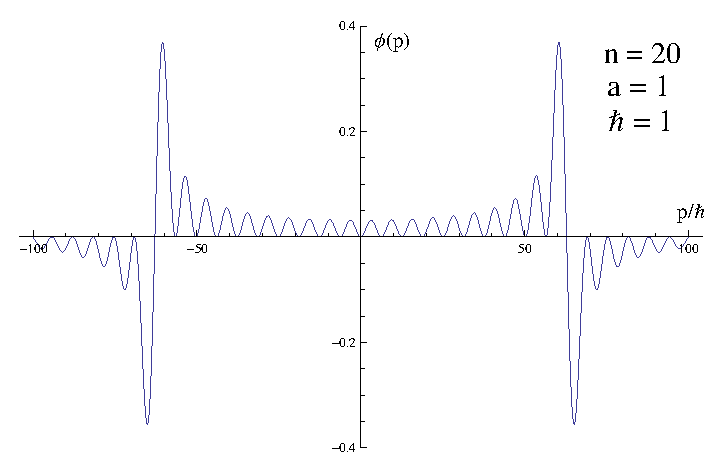
\includegraphics[width=300pt,height=200pt]{phi_p.eps}\\
      \caption{$\varphi(p)$}
    \end{figure}
    }\\[20pt]  
    \noindent 2.5 \textbf{解:}\\[12pt]
    {
    根据2.2中结果,将$a\rightarrow 2a$可得
    $$\psi_{n}(x) = \sqrt{\frac{1}{a}}\sin (\frac{n\pi x}{2a})\quad , \quad E_{n} = \frac{n^{2}\pi_{2}\hbar^{2}}{8 m a^{2}}$$
    故$\psi(x,0)$不是能量本征态,但恰有$\displaystyle E_{1}=\frac{\pi^{2}\hbar^{2}}{2 m a^{2}}=\epsilon_{2}$,
        将$\psi(x,0)$用$\psi_{n}(x)$展开,即$\psi (x,0) = \sum C_{n} \psi_{n}(x)$,其中:
    \begin{eqnarray}
    C_{n}  & = &  \int \psi_{n}^{*} (x) \psi (x) \mathrm{d x} 
        = \int_{0}^{a} \sqrt{\frac{2}{a}}\sin (\frac{\pi x}{a})\sqrt{\frac{1}{a}}\sin (\frac{n\pi x}{2a})\mathrm{d x}\nonumber\\
        & = & \frac{4\sqrt{2}}{(4 - n^{2})\pi}\sin(\frac{n\pi}{2})
        \quad (\psi(x,0)=0,x<0 \bigcup x>a )\nonumber    
    \end{eqnarray}
    求测得粒子能量仍为$E_{1}$的概率
    $$P = |C_{2}|^{2} = |\lim_{n\rightarrow 2} C_{n}|^{2} = \frac{1}{2}.$$
    }    
    \end{CJK*}
    \begin{CJK*}{UTF8}{kai}
        \begin{flushright}
            \small PB12203077\quad吴奕涛\\
            \small \today
        \end{flushright}
    \end{CJK*}

\end{document} 